\section{Overview of KIDs}
\label{sec2}
\subsection{KID physics}

Kinetic inductance detectors are a novel superconducting detector technology that provides high sensitivity and ease of multiplexing. In this section we give a brief summary of the main features of KIDs.\\
KIDs are RLC superconducting resonators made from a thin metal film that react to an incoming radiation by changing their electromagnetic properties. In fact, when photons are absorbed by the superconducting film, they break Cooper pairs which increases the quasi-particles density and causes a change in the kinetic inductance $L_{k}$. This produces a shift, $\delta f_{0}$, of the resonant frequency of the KID \citep{2013A&A...551L..12C} that can be related to the absorbed optical power $\delta P_{opt}$. This relation is linear for small variations in $P_{opt}$ \citep{2010ApPhL..96z3511S}. The operating principle is represented in Fig.~\ref{resonance}.\\

\begin{figure}[h]
\center
	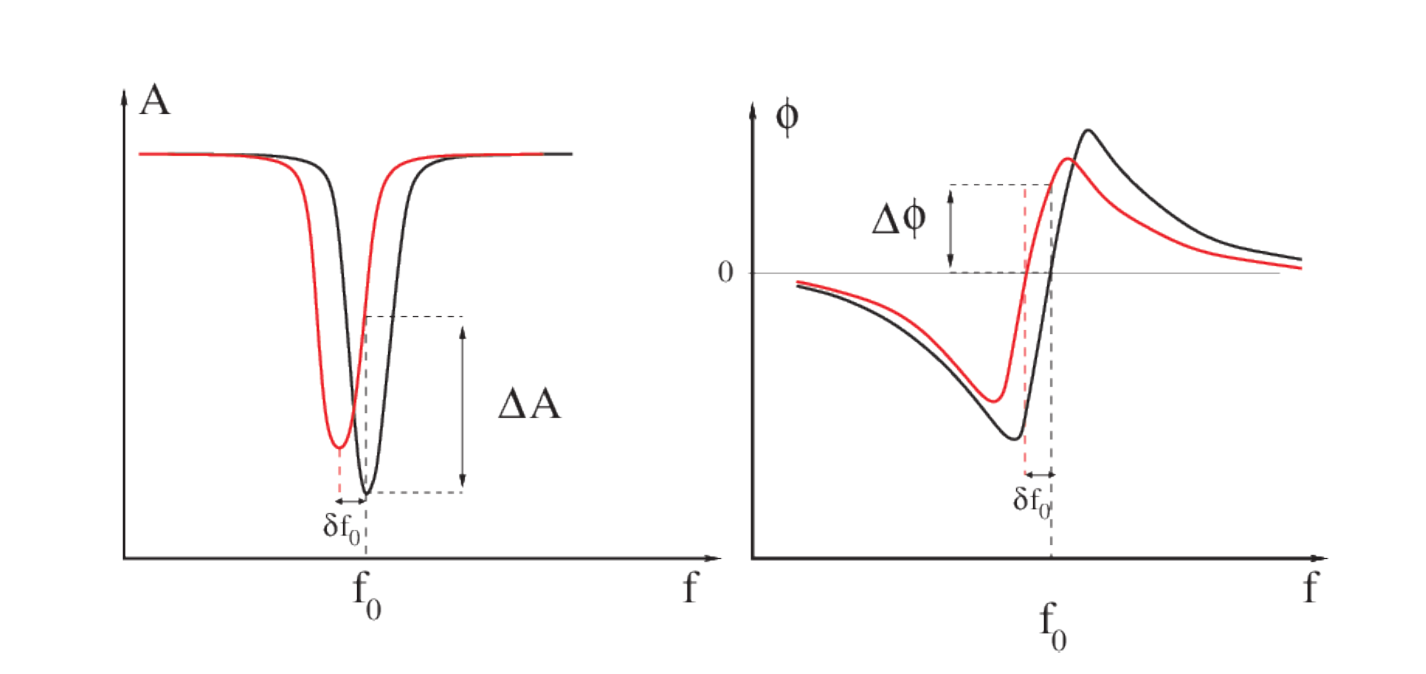
\includegraphics[scale=0.4]{Figures/resonance.png}
	\caption{Schematic representation of a KID resonance in amplitude (left) and phase (right), as a function of the excited tone injected in the feedline. The optical power absorbed by the detector is weak for black curves and increases for red curves. The absorption of a photon shifts the resonance frequency and this is directly proportional to the received power.}
	\label{resonance}
\end{figure}

The KID transfer function is given by :

\begin{equation}
S_{21}(f) = I +jQ .
\end{equation}

where \I\  and \Q\  give respectively the real (in phase) and imaginary (quadrature) of $S_{21}$.

\subsection{KID model}
A model of a KID transfer function has been proposed by \citet{2008ApPhL..93m4102G} :

\begin{equation}
S_{21} = \frac{2Z_{res}Z_{0}}{Z_{res}[2Z_{0} + j(X_{1}+X_{2})] + (Z_{0} +jX_{1})(Z_{0} +jX_{2})},
\end{equation}

with :

\begin{equation}
Z_{res} = \frac{Z_{0}Q_{e}}{2Q_{i}}[1 + 2jQ_{i}\frac{(f-f_{0})}{f_{0}}],
\end{equation}

where $X_{1}$, $X_{2}$, $Z_{0}$ are impedances, $Q_{i}$ is the intrinsic quality factor of the resonator and $Q_{e}$ is the external quality factor due to coupling with the measurement electronics. $f$ is the frequency of excitation of the detector, and $f_{0}$ is the resonant frequency. Throughout this paper, we shall assume typical values of KIDs $X_{1} = X_{2} = 3 $ $\Omega $, $Z_{0} = 50$ $\Omega$, $Q_{i} \simeq 5.10^{4}$, $Q_{e} \simeq 2.10^{4}$ and $f_{0} = 1.273$x$10^{9}$ Hz measured on \nika\ and \nikad. \\

In order to reconstruct the incident optical power on the KID, two methods were developed and are presented in the following section.
